Every chapter so far has asked how the model handles one task. But real
capability isn't learned in one shot --- it's \emph{grown}, by adding
new things over time. That raises the question at the heart of continual
learning: when we teach a model something new, does the new thing stick
--- and does the model \textbf{keep} the old things?

There's a well-known failure mode with a scary name:
\textbf{catastrophic forgetting} --- the tendency of a model, after
training on task B, to lose what it learned on task A. We want to know
whether that happens to our small model, and, crucially, whether the
\emph{way} we train determines it.

It is like learning a new language. Study French for a year, then stop
and study Spanish exclusively --- how much French is left? A lot depends
on whether French keeps being practiced while Spanish is learned ---
which is exactly what this experiment tests. And it is a question almost
every learning system faces: a deployed model is rarely trained once and
frozen. It is updated, re-trained, fine-tuned on new data. So whether it
\emph{keeps} what it knew is a practical concern, not an academic one.

\section{The setup}\label{the-setup}

We split the operations into two capabilities:

\begin{itemize}
\tightlist
\item
  \textbf{Capability A --- arithmetic:} \texttt{add}, \texttt{sub},
  \texttt{mul}, \texttt{max\_of}, \texttt{min\_of}.
\item
  \textbf{Capability B --- lists:} \texttt{list\_sum},
  \texttt{list\_len}, \texttt{first\_element}.
\end{itemize}

We train on A, then introduce B, and measure both: - \textbf{B
acquisition} --- did it learn the new capability? - \textbf{A retention}
--- did it keep the old one, or did learning B destroy it?

This double measurement is the crux of the design. Many
continual-learning reports measure only whether the model acquired the
\emph{new} task, and that alone can make the whole thing look like a
success. But the interesting failure is usually what was \emph{lost} to
get there. So we insist on measuring both, every time.

We run this under two protocols, changing only the \emph{order and
mixing}, not the model, data, or optimizer:

\begin{itemize}
\tightlist
\item
  \textbf{sequential:} learn A fully, then learn B with no A exposure.
\item
  \textbf{replay / mixed:} interleave A and B examples throughout.
\end{itemize}

Holding model, data, and optimizer constant while changing only the
training \emph{schedule} is a textbook application of our one-variable
discipline. If the results differ between the two protocols, the
difference cannot be attributed to the model, the data, or the optimizer
--- it must be the schedule. That makes any difference we find a
\emph{procedure} finding, exactly the thing we want to isolate.

\section{The result}\label{the-result}

\begin{figure}
\centering
\pandocbounded{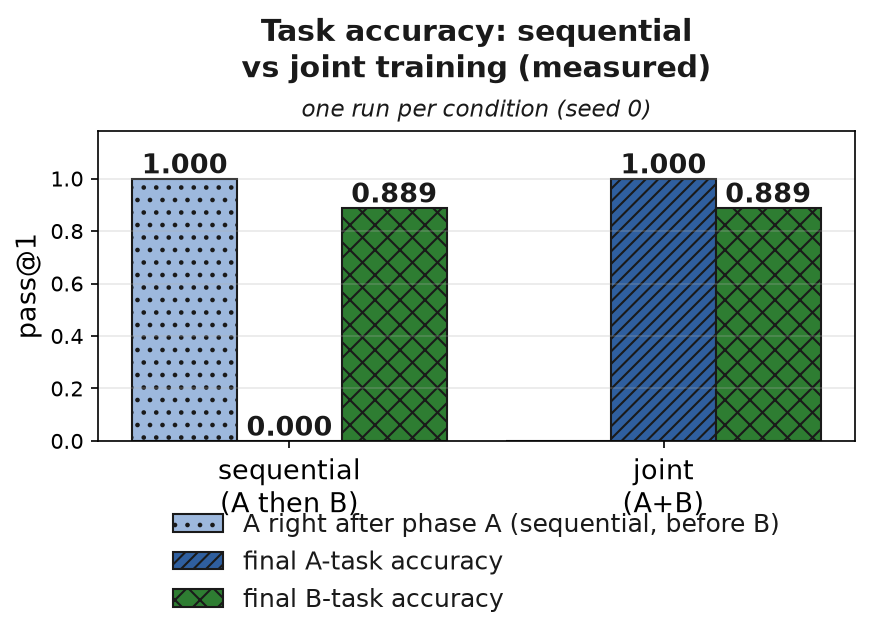
\includegraphics[keepaspectratio,alt={Continual learning},width=\maxwidth{\textwidth},keepaspectratio]{figures/fig_continual.png}}
\caption{Continual learning}
\end{figure}

\begin{longtable}[]{@{}lll@{}}
\toprule\noalign{}
Protocol & \textbf{A-retention} & \textbf{B-acquisition} \\
\midrule\noalign{}
\endhead
\bottomrule\noalign{}
\endlastfoot
\textbf{sequential} & \textbf{0.000} & 0.889 \\
\textbf{replay} & \textbf{1.000} & 0.889 \\
\end{longtable}

This is as clean a result as this book produced.

\textbf{Sequential training causes catastrophic forgetting.} After
learning arithmetic and then lists in sequence, the model's A-retention
is \textbf{0.000} --- it completely forgot the first capability. That is
not ``degraded''; it is gone. Learning the lists overwrote the
arithmetic.

\textbf{Replay prevents it, with zero cost.} When A and B are
interleaved throughout, the model's A-retention is a perfect
\textbf{1.000}, and B-acquisition is \textbf{0.889} --- identical to
sequential. So replay bought complete retention of the old capability
with \textbf{no trade-off whatsoever} in learning the new one.

\section{Why this result is so
striking}\label{why-this-result-is-so-striking}

The symmetry is what makes this remarkable. Under sequential training,
the model forgets A completely (0.000) but learns B fine (0.889). Under
replay, it keeps A perfectly (1.000) \emph{and} learns B just as well
(0.889). Nothing about the model, the data, or the optimizer changed ---
only whether the old examples stayed in the mix while the new ones were
learned.

This is the clearest case in the book where the \textbf{training
protocol, not the model or the data, determines the outcome.} Same
model. Same data. Same optimizer. The only difference is whether the
first capability stays ``in the mix'' while the second is learned.
Sequential forgets; replay retains.

There is an intuition that makes this easy to see. Imagine a muscle
being trained on exercise A. If it then trains exclusively on exercise B
and never revisits A, the muscle's adaptation to A fades. But if A and B
alternate, both stay. The model's weights are like that muscle --- the
gradient signal from new examples keeps pushing them, and if nothing
pulls them back toward the old behavior, the old behavior erases. Replay
is simply making sure the old examples are still in the rotation.

The lesson generalizes directly: when a new capability is added to a
model, \emph{how} it is done matters more than any property of the model
itself. If the new task is allowed to dominate the gradient signal and
the old data is removed, the old capability collapses. If old and new
stay interleaved, the model can hold both.

\section{Reframing a common
assumption}\label{reframing-a-common-assumption}

And it reframes a common assumption. People often reach for ``a bigger
model'' when confronted with a model that forgets. This experiment shows
the forgetting was never a capacity problem --- a \textasciitilde0.9M
model holds both capabilities perfectly under replay. It was a
\emph{training procedure} problem. Here, as with composition, the
instinctive fix (``make it bigger'') would have been exactly wrong.

The pattern here echoes a deeper truth we've seen all book: the headline
number (``did it learn the new thing?'') hides the interesting failure
(``what did it lose to get there?''). Measuring B acquisition alone
would have made sequential training look like a success --- 0.889,
great. Measuring A retention reveals the cost. The lesson is to always
measure \emph{both} the new and the old.

\section{The shortcut audit}\label{the-shortcut-audit}

\begin{enumerate}
\def\labelenumi{\arabic{enumi}.}
\tightlist
\item
  \textbf{Suspected shortcut: the 0.000 A-retention is an artifact of
  how we score A.} \textbf{Why it could explain it:} maybe the A test is
  too hard, or the model just needs more steps. \textbf{Control:} replay
  mode, identical A test --- A-retention 1.000. \textbf{What it rules
  out:} a broken A test. The same test that scores 0.000 in sequential
  scores 1.000 in replay. \textbf{What remains:} whether this holds for
  three or more capabilities, and whether replay-adds support
  \emph{composition} of A and B after the fact.
\end{enumerate}

\section{The honest summary}\label{the-honest-summary}

Acquiring a new capability can destroy an old one --- and it is entirely
up to how we train. Sequential training forgets; replay retains with no
cost. This is a controlled, reproducible demonstration that catastrophic
forgetting is a procedure problem, and it is one of the most practically
useful results in the book.

What makes it feel like a real discovery is that the right answer was
sitting in a choice we made near-automatically. When we first set up the
experiment, sequential training was the path of least resistance ---
learn one thing, then the next. The surprise came from asking the
question we almost didn't ask: what did the model lose to learn the new
thing? And the fix --- just keeping old examples in the mix --- was so
simple it was almost anticlimactic. But that simplicity is the point.
Sometimes the most important finding in an experiment is not a complex
technique but a simple change to the way we were already working.
